\chapter{Tests and Results}

\paragraph{}
The Question Answer System implemented is part of the Yioop search engine and is platform independent. The system works by tagging phrases using a Brill variant Part of Speech tagger for Hindi sentences. In the next step, triplets are formed and stored in the database using the grammar rules for Hindi. The test data for the system is an index created by configuring Yioop to crawl hindi webpages from Wikipedia and Indian websites with Hindi content. We created 3 crawls about 100,000 webpages from which the summarizer extracted text from 6000 documents to create the index. Below are examples, of some 'Wh' questions to the system.

\section {Standalone Testcase}
In this section, we provide a text case for the system as standalone module. It is assumed that the input to the system is a semantically and syntactically correct sentence.

\begin{enumerate}
\item  Figure 9 shows the sentence after it is tagged for parts of speech

\begin{figure}[htb]
\centering
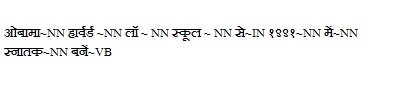
\includegraphics[width=0.8\textwidth]{images/sentence_testcase1.jpg}
\caption{Standalone Sentence 1.} 
\label{fig:sentence_testcase1}
\end{figure}

A word for word translation of the above sentence to English is 'Obama Harward law school from 1999 graduate complete'. From the translation, we can guess which words should go into the noun, post and verb phrases. Figure 10 shows the Parse Tree generated for this sentence 

\begin{figure}[htb]
\centering
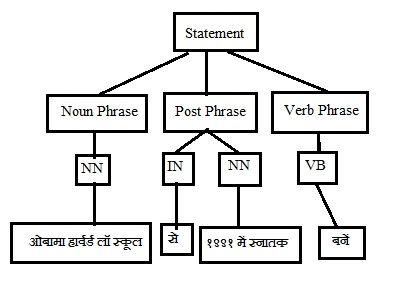
\includegraphics[width=0.8\textwidth]{images/standalone_testcase.jpg}
\caption{Parse Tree for sentence in Figure 9.} 
\label{fig:standalone_testcase}
\end{figure}

\paragraph{}
The triplets extracted for the above parse tree are as shown in Figure 11 above.

\begin{figure}[htb]
\centering
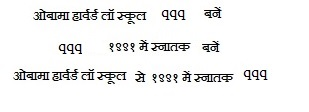
\includegraphics[width=0.8\textwidth]{images/triplet_standalone.jpg}
\caption{Triplets Extracted for sentence Figure 9.} 
\label{fig:triplet_standalone}
\end{figure}

\break
\item  Figure 12 shows the sentence after it is tagged for parts of speech

\begin{figure}[htb]
\centering
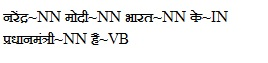
\includegraphics[width=0.5\textwidth]{images/sentence_testcase2.jpg}
\caption{Standalone Sentence 2.} 
\label{fig:sentence_testcase2}
\end{figure}

A word for word translation of the above sentence to English is 'Narendra Modi India (s) Prime Minister is'. From the translation, we can guess which words should go into the noun, post and verb phrases. Figure 13 shows the Parse Tree generated for this sentence 

\begin{figure}[htb]
\centering
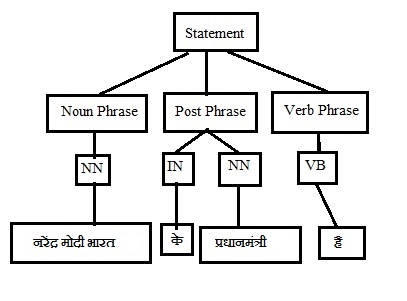
\includegraphics[width=0.8\textwidth]{images/standalone_testcase2.jpg}
\caption{Parse Tree for sentence in Figure 12.} 
\label{fig:standalone_testcase2}
\end{figure}

\end{enumerate}

\break
\section{Question Answer Module Integrated in Yioop}
\paragraph{}
Below are results for the Question Answer System when a crawl was setup for all wikipedia pages in Hindi, Indian websites. The crawler was able to crawl 100,000 webpages and extract information from 5925 webpages to create the index. Figure 14, Figure 15 and Figure 16 are examples of Who, Why and What questions and with the best answer displayed at the top.

\begin{figure}[htb]
\centering
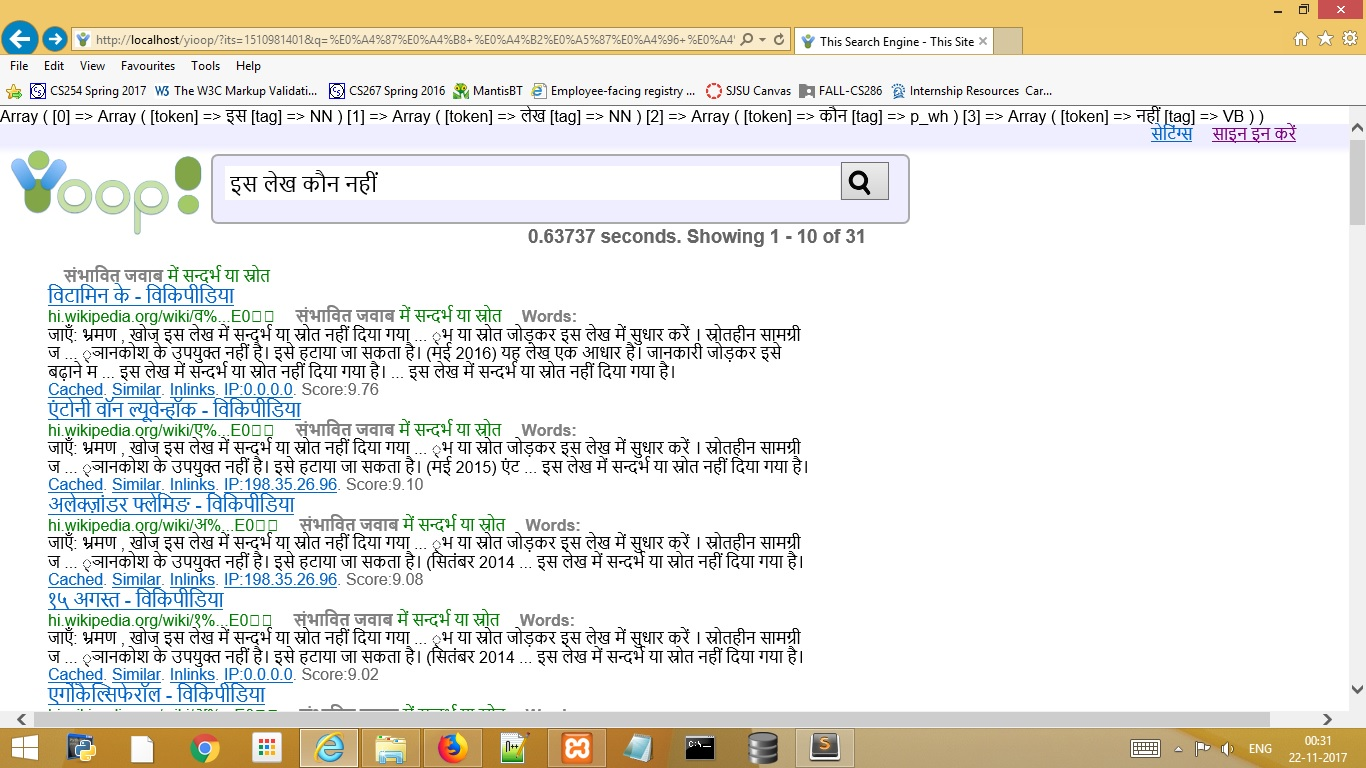
\includegraphics[width=0.8\textwidth]{images/who_question.jpg}
\caption{Who Question.} 
\label{fig:who_question}
\end{figure}

\begin{figure}[htb]
\centering
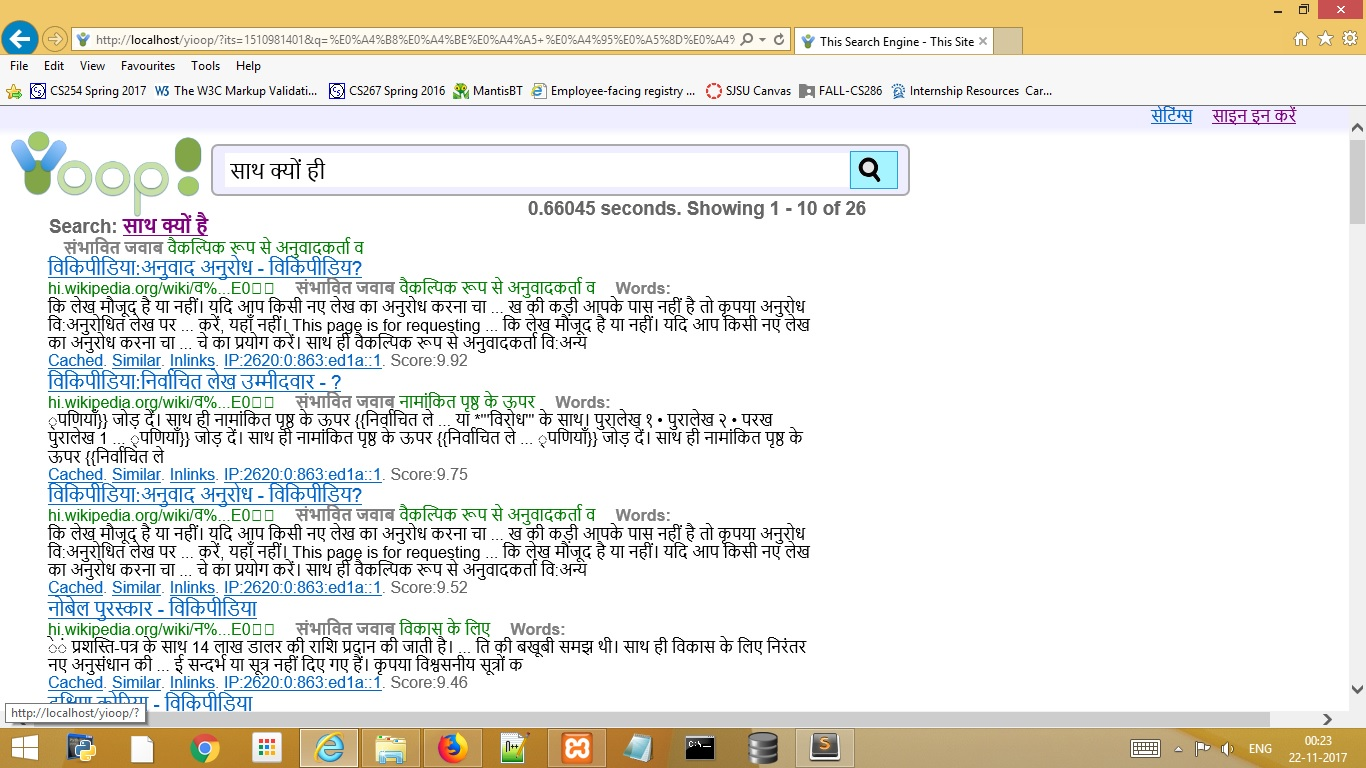
\includegraphics[width=0.8\textwidth]{images/why_question.jpg}
\caption{Why Question.} 
\label{fig:why_question}
\end{figure}

\begin{figure}[htb]
\centering
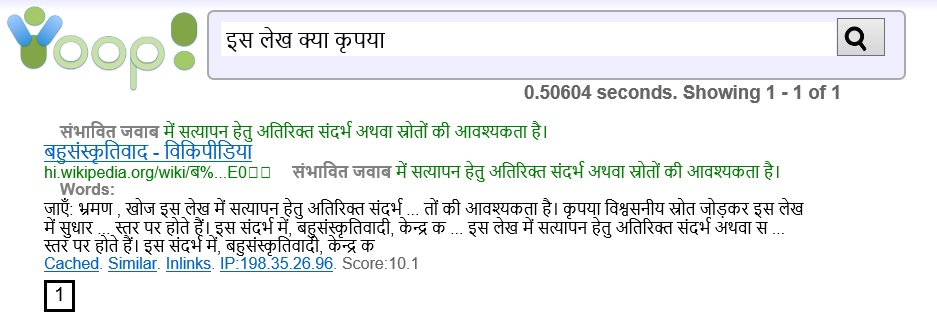
\includegraphics[width=0.8\textwidth]{images/what_question.jpg}
\caption{What Question.} 
\label{fig:what_question}
\end{figure}